% !TEX encoding = UTF-8
% !TEX TS-program = pdflatex
% !TEX root = ../tesi.tex

%**************************************************************
\chapter{Data collection}
\label{cap:analisi-requisiti}
%**************************************************************

\intro{This chapter gives an overview of the data collection process, which finished with the creation of the logs that we used as base for our work.\\ 
In section \ref{sec:fi} we present the process of finding the data, in section \ref{sec:do} we look at the way the matches were downloaded, and in section \ref{sec:pa} we explore the parsing.}

%***************************************************************

\section{\label{sec:fi}Finding the data}

	The first step of the data collection was to find a tracking website that could provide the replays of the matches. 
	For this purpose, the two websites considered are csgostats\footnote{\href{https://csgostats.gg/}{https://csgostats.gg/}} and hltv\footnote{\href{https://www.hltv.org/}{https://www.hltv.org/}}.
	In the beginning, csgostats seemed a better choice, so, looking through the players, 50 of them were selected. 
	Every selected player must have played at least 100 matches as the minimum requirement. 
	After we found the profiles, we tried to create a script to download the matches automatically. 
	The problem was that there is the invisible reCAPTCHA, so we decided to use hltv, which does not use these codes. 
	After that, we checked if the players selected were present in hltv. 
	We then replaced the players that were not present on this website with other players that we found. 
	As the final step, we wrote all the links to the profiles of the players on hltv on a \emph{txt} file.

\section{\label{sec:do}Getting the data}

	For every player we found, we had to download 100 matches. 
	We found a way to automate the download process with a python script and the framework Selenium\footnote{\href{https://www.selenium.dev/}{https://www.selenium.dev/}}. 
	Using Selenium's Chrome web driver, we downloaded all the matches starting from the profile page of one player at a time. 
	The download starts when the web driver performs a request, via Selenium's get method, to a link for the direct download of the replay. 
	The download result is a compressed file that gets unpacked using the pyunpack module\footnote{\href{https://github.com/ponty/pyunpack/tree/0.2.2}{https://github.com/ponty/pyunpack/tree/0.2.2}}. 
	The extracted files get counted and renamed to keep track of how many matches remain to reach 100. 
	Finally, the compressed archives get deleted from the pc.

\section{\label{sec:pa}Parsing the matches}

	The parsing process is divided into two parts: the modification of the parser itself to parse what we needed and the automation of the parsing process.
	To parse the data we needed, we first found an already existing parser. 
	The mentioned parser is called demoinfogo and is an open-source software developed by Valve. 
	In the beginning, we parsed a match with the original parser to see the result. 
	Then we modified the outputs to trace the origin of every line in the output file. 
	After that, we changed the parser, silencing what we did not need and writing in a file everything relevant for our task. 
	Lastly, we wrote a python script that helped us automatically parse all the matches and rename all the files with the corresponding player's name. 
	These files created by the parser are the logs we used as starting point in this work.

	In more detail, the fundamental unit of the replay is the \gls{tick}, and the parser dumps the state of every player and every action occurred during the tick with the related informations. 
	So, the parsed replay can be seen as a sequence of states dumped by the parser. 
	The states can include both player information and actions informations.
	Figure \ref{fig:act} presents an example of parsed action.
	
	\begin{figure}[!h] 
		\centering 
		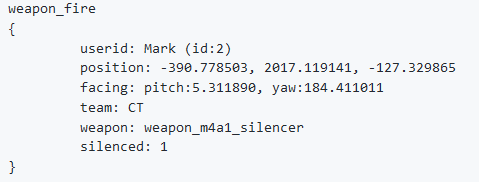
\includegraphics[width=.9\columnwidth]{parser/original_action.png}
		\caption{\label{fig:act}Example of parsed action.}
	\end{figure}
	
	Given this, we used the parser to dump only a set of features (shown in Table \ref{tab:fea}) of the player we were interested in.
	
	\begin{table}
	
		\caption{\label{tab:fea}List of parsed features}
		\centering
		\begin{tabular}{|c|c|}
		
			\hline
			\textbf{Type} & \textbf{Features}\\
			\hline
			Camera & X, Y \\
			\hline
			Player position & X, Y, Z \\
			\hline
			door\_moving & occurred \\
			\hline
			player\_blind & occurred, blind\_duration \\
			\hline
			round\_mvp & occurred \\
			\hline
			defuser\_pickup & occurred \\
			\hline
			bomb\_pickup & occurred \\
			\hline
			defuser\_dropped & occurred \\
			\hline
			bomb\_dropped & occurred \\
			\hline
			bomb\_abortdefuse & occurred \\
			\hline
			bomb\_begindefuse & occurred \\
			\hline
			bomb\_abortplant & occurred \\
			\hline
			bomb\_beginplant & occurred \\
			\hline
			bomb\_defused & occurred \\
			\hline
			bomb\_planted & occurred \\
			\hline
			bullet\_impact & occurred \\
			\hline
			weapon\_zoom & occurred \\
			\hline
			weapon\_zoom\_rifle & occurred \\
			\hline
			player\_falldamage & occurred, damage\\
			\hline
			molotov\_detonate & occurred \\
			\hline
			tagrenade\_detonate & occurred \\
			\hline
			hegrenade\_detonate & occurred \\
			\hline
			flashbang\_detonate & occurred \\
			\hline
			item\_purchase & occurred, item\_purchased \\
			\hline
			ammo\_pickup & occurred \\
			\hline
			silencer\_detach & occurred \\
			\hline
			decoy\_detonate & occurred \\
			\hline
			smokegrenade\_detonate & occurred \\
			\hline
			weapon\_fire & occurred, weapon \\
			\hline
			weapon\_reload & occurred \\
			\hline
			player\_jump & occurred \\
			\hline
			player\_death & occurred, type (kill, death, or assist)\\
			\hline
			item\_pickup & occurred, item\_picked \\
			\hline
			item\_equip & occurred, item\_equipped\\
			\hline
	
		\end{tabular}
	
	\end{table}

	In this way, viewing the replay as a sequence of states and the parser as a program used to dump those states, we could parse the replays.
	So, the parser dumps the replays in a predefined way, following this structure:
	
	\begin{itemize}
	
		\item If the parser has to dump an action, it writes the word Action, the tick when the action occurred, the action name, and then the additional informations (if present)
		\item If the parser has to dump the player's state, it writes the word Entity, the current tick, the mouse position ($X$ and $Y$), the player's position in the map ($X$, $Y$, and $Z$), 
		the player's velocity ($X$, $Y$, and $Z$), and the Y offset (used to determine the crouch state).
	
	\end{itemize}
	
	In Figure \ref{fig:parsed} there is an example of a parsed match.
	
	\begin{figure}[!h] 
		\centering 
		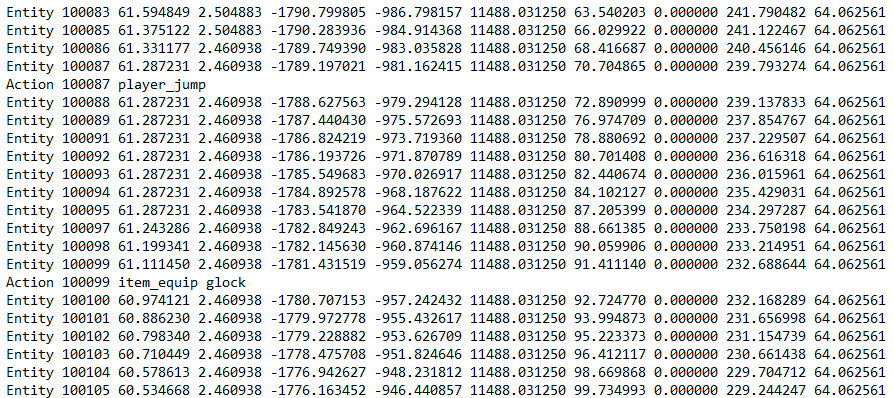
\includegraphics[width=0.9\columnwidth]{parser/log.png}
		\caption{\label{fig:parsed}Parsed replay fragment.}
	\end{figure}

	For more details on the parser see appendix \ref{app:par}
